\chapter[Analysis]{Analysis}

\section{Overview}
While Figure \ref{fig:alldata-GOES6-1983-1991} shows an overview of the most pertinent variables used in this study, some further analysis was done to determine any potential biases introduced by specifics of the satellite motion or derivations used. For example, Figure \ref{fig:ByHourExample} shows that not only did data availability vary significantly with magnetic local time (MLT), but the values themselves vary significantly (e.g. AE models are better in the dawn sector and \dst\ models better at dusk \citep{OBrien2003EmpiricalPlasmapause}. \vinote{Go as far back as Carpenter 1967? http://adsabs.harvard.edu/abs/1967JGR....72.2969C Yes, but put earlier in paragraph}

\begin{figure}[htp!]
\centering
\includegraphics[width=0.7\linewidth]{Figures/rhoMLT.eps}
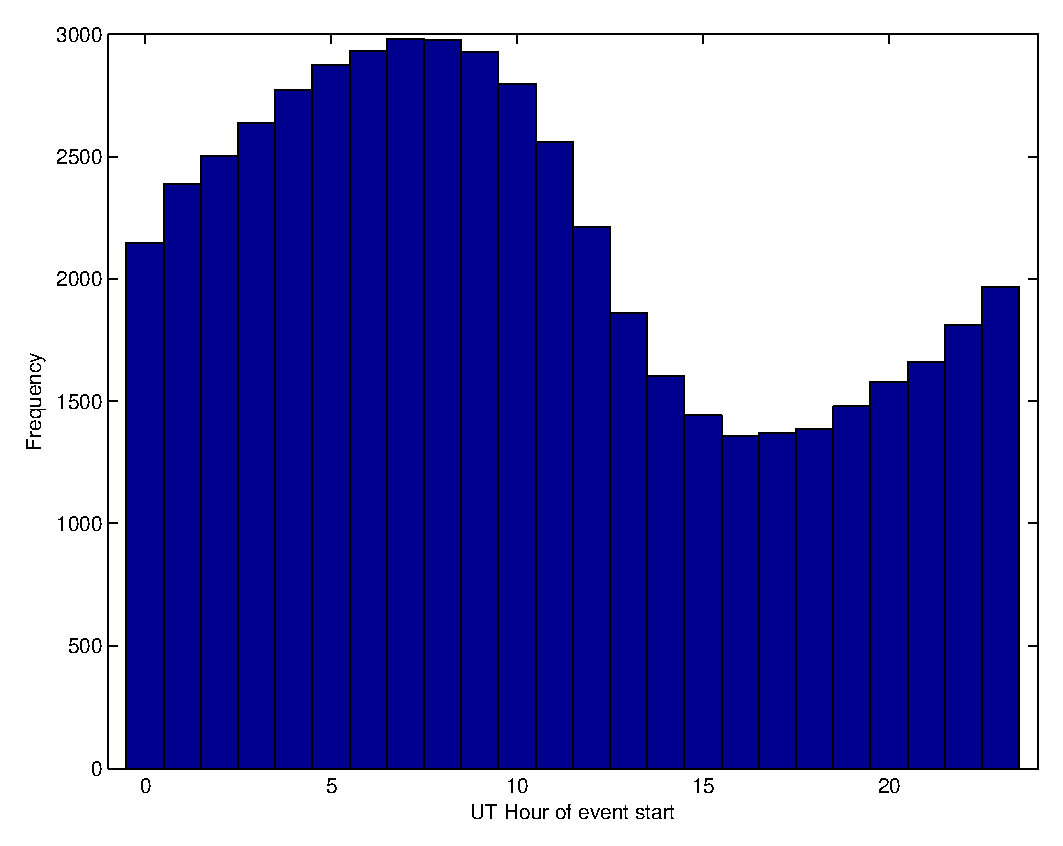
\includegraphics[width=0.7\linewidth]{Figures/nansbyhour.eps}
\caption{Median \req\ binned by local time, and availability of \req\ with local time.}
\label{fig:ByHourExample}
\end{figure}


\section{Linear Correlations}
This dependence was further investigated, and extended, by creating a simple linear model for each major variable in the database as well as combinations of some to investigate independent contributions to the total correlation (by testing how much correlation improved in a combined model over either of the constituent models.)  The inputs were the median values of each variable for four hours before a \dst\ event onset, and they were trained to predict a median of the value at onset with the four hours following it. The models were trained on half of the dataset and tested on the other half for each satellite, and this was repeated with new random samples 100 times and then the median correlation values were taken. The results are shown in Table \ref{CCperltable}.


\begin{table}[h]
	\small
	\begin{tabular}{|L|LLLL|}
		\hline
		& \text{GOES 2} & \text{GOES 5} & \text{GOES 6} & \text{GOES 7}\\ \hline
		DoY & -0.08\pm0.08 & +0.14\pm0.13 & -0.06\pm0.06 & +0.09\pm0.10 \\
		MLT & -0.10\pm0.21 & -0.07\pm0.12 & +0.01\pm0.23 & -0.06\pm0.05 \\
		B_z & +0.16\pm0.21 & -0.13\pm0.15 & +0.08\pm0.14 & -0.07\pm0.06 \\
		V_{sw} & -0.04\pm0.10 & +0.27\pm0.09 & +0.06\pm0.11 & -0.06\pm0.06 \\
		D_{st} & +0.26\pm0.17 & +0.66\pm0.08 & +0.06\pm0.13 & +0.23\pm0.14 \\
		\rho_{sw} & +0.35\pm0.24 & +0.63\pm0.31 & +0.12\pm0.19 & +0.36\pm0.17 \\
		F_{10.7} & +0.43\pm0.08 & +0.12\pm0.12 & +0.51\pm0.06 & +0.40\pm0.06 \\
		B_z+V_{sw} & +0.11\pm0.17 & +0.20\pm0.17 & +0.12\pm0.10 & -0.12\pm0.06 \\
		D_{st}+F_{10.7} & +0.44\pm0.09 & +0.71\pm0.08 & +0.54\pm0.07 & +0.47\pm0.06 \\
		All & -0.03\pm0.19 & +0.34\pm0.27 & +0.61\pm0.11 & +0.40\pm0.12 \\
		\hline
	\end{tabular}
	\caption{Table of linear model correlations showing the median of 100 random samples. Each sample trained on half of the data (via randomly selected rows of the least squares matrix) and tested on the other half} 
	\label{CCperltable}
\end{table}

 \begin{table}[h]
 	\small
 	\begin{tabular}{|L|LLLL|}
 		\hline
 		T-Tr & \text{GOES 2} & \text{GOES 5} & \text{GOES 6} & \text{GOES 7}\\ \hline
 		DoY & -0.16\pm+0.11 & -0.02\pm+0.16 & -0.12\pm+0.08 & +0.01\pm+0.12 \\
 		MLT & -0.26\pm+0.25 & -0.16\pm+0.14 & -0.16\pm+0.26 & -0.11\pm+0.07 \\
 		B_z & -0.06\pm+0.24 & -0.27\pm+0.18 & -0.05\pm+0.17 & -0.14\pm+0.08 \\
 		V_{sw} & -0.11\pm+0.13 & -0.02\pm+0.13 & -0.03\pm+0.13 & -0.12\pm+0.08 \\
 		D_{st} & -0.02\pm+0.21 & -0.01\pm+0.12 & -0.06\pm+0.16 & +0.00\pm+0.17 \\
 		\rho_{sw} & -0.01\pm+0.29 & -0.01\pm+0.37 & -0.04\pm+0.22 & +0.03\pm+0.21 \\
 		F_{10.7} & +0.01\pm+0.11 & -0.04\pm+0.16 & +0.00\pm+0.08 & -0.03\pm+0.08 \\
 		B_z+V_{sw} & -0.15\pm+0.20 & -0.17\pm+0.20 & -0.08\pm+0.12 & -0.24\pm+0.08 \\
 		D_{st}+F_{10.7} & -0.05\pm+0.12 & +0.02\pm+0.11 & -0.01\pm+0.10 & -0.03\pm+0.08 \\
 		All & -0.64\pm+0.22 & -0.54\pm+0.28 & -0.16\pm+0.14 & -0.25\pm+0.13 \\
 		\hline
 	\end{tabular}
 	\caption{Table of differences in linear testing-training models, where each correlation is the median correlation of 100 random samples. Each sample trained on half of the data (via randomly selected rows of the least squares matrix) and tested on the other half} 
 	\label{CCdifftable}
 \end{table}




It can be seen that $F_{10.7}$ almost always correlates the best with \req, but that there is significant variance between data from different satellites. 

\section{Nonlinear Correlations}

Similarly for a neural net model with the same input and target structure as the linear model, but training on a randomly selected 70\% of the data, testing on another 15\%, and validating on the remaining 15\%, Table \ref{NNperltable} shows the resulting correlation values for the validation data set.

 \begin{table}[h]
 	\small
 	\begin{tabular}{|L|LLLL|}
 		\hline
 		& \text{GOES 2} & \text{GOES 5} & \text{GOES 6} & \text{GOES 7}\\ \hline
 		DoY & +0.05\pm0.31 & +0.31\pm0.30 & +0.32\pm0.22 & +0.12\pm0.17 \\
 		MLT & +0.29\pm0.41 & +0.15\pm0.34 & +0.40\pm0.32 & +0.17\pm0.21 \\
 		B_z & +0.24\pm0.23 & +0.21\pm0.28 & +0.17\pm0.19 & -0.00\pm0.20 \\
 		V_{sw} & +0.20\pm0.25 & +0.36\pm0.19 & +0.19\pm0.24 & +0.06\pm0.18 \\
 		D_{st} & +0.08\pm0.27 & +0.18\pm0.25 & +0.02\pm0.17 & +0.18\pm0.24 \\
 		\rho_{sw} & +0.02\pm0.29 & +0.25\pm0.42 & +0.20\pm0.22 & +0.12\pm0.29 \\
 		F_{10.7} & +0.26\pm0.27 & +0.32\pm0.29 & +0.48\pm0.25 & +0.36\pm0.15 \\
 		B_z+V_{sw} & +0.11\pm0.25 & +0.20\pm0.38 & +0.15\pm0.21 & +0.02\pm0.17 \\
 		D_{st}+F_{10.7} & +0.17\pm0.25 & +0.21\pm0.32 & +0.47\pm0.15 & +0.35\pm0.17 \\
 		All & +0.21\pm0.41 & +0.67\pm0.40 & +0.60\pm0.35 & +0.17\pm0.33 \\
 		\hline
 	\end{tabular}
 	\caption{Table of nonlinear model test correlations showing the median of 100 random samples. Each sample trained on half of the data (via randomly selected rows of the least squares matrix) and tested on the other half} 
 	\label{NNperltable}
 \end{table}
 
 
 
 \begin{table}[h]
 	\small
 	\begin{tabular}{|L|LLLL|}
 		\hline
 		T-Tr & \text{GOES 2} & \text{GOES 5} & \text{GOES 6} & \text{GOES 7}\\ \hline
 		DoY & -0.16\pm+0.11 & -0.02\pm+0.16 & -0.12\pm+0.08 & +0.01\pm+0.12 \\
 		MLT & -0.26\pm+0.25 & -0.16\pm+0.14 & -0.16\pm+0.26 & -0.11\pm+0.07 \\
 		B_z & -0.06\pm+0.24 & -0.27\pm+0.18 & -0.05\pm+0.17 & -0.14\pm+0.08 \\
 		V_{sw} & -0.11\pm+0.13 & -0.02\pm+0.13 & -0.03\pm+0.13 & -0.12\pm+0.08 \\
 		D_{st} & -0.02\pm+0.21 & -0.01\pm+0.12 & -0.06\pm+0.16 & +0.00\pm+0.17 \\
 		\rho_{sw} & -0.01\pm+0.29 & -0.01\pm+0.37 & -0.04\pm+0.22 & +0.03\pm+0.21 \\
 		F_{10.7} & +0.01\pm+0.11 & -0.04\pm+0.16 & +0.00\pm+0.08 & -0.03\pm+0.08 \\
 		B_z+V_{sw} & -0.15\pm+0.20 & -0.17\pm+0.20 & -0.08\pm+0.12 & -0.24\pm+0.08 \\
 		D_{st}+F_{10.7} & -0.05\pm+0.12 & +0.02\pm+0.11 & -0.01\pm+0.10 & -0.03\pm+0.08 \\
 		All & -0.64\pm+0.22 & -0.54\pm+0.28 & -0.16\pm+0.14 & -0.25\pm+0.13 \\
 		\hline
 	\end{tabular}
 	\caption{Table of differences in linear testing-training models, where each correlation is the median correlation of 100 random samples. Each sample trained on half of the data (via randomly selected rows of the least squares matrix) and tested on the other half \vinote{No plus on error, do tr-t. Center headers.}} 
 	\label{CCdifftable}
 \end{table}

  
 

It should be noted that nonlinear modeling is much more susceptible to overfitting than linear modeling \vinote{cite?} due to the higher order of fitting done on training and validation data, as well as the lack of a straight-forward optimal error-minimization method such as least squares regression \vinote{(non-unique solution, non-guaranteed convergence, etc)}. This is why some models, such as that including every possible variable, correlate worse than models of just a few parts. Where a linear model can minimize error by zeroing out variables without useful information, the neural net will try to incorporate the information anyway and end up overfitting. Table \ref{NNdifftable} shows how significant the differences are between training data and testing data by subtracting the median correlations from both data sets from each other, and doing the root mean squared (RMS) error as the combination of the two constituent errors.



\section{$F_{10.7}$ Dependence}
\cite{Takahashi2010SolarCycleVariation} showed a strong correlation between the 27-day averaged $F_{10.7}$ index of solar activity and the averaged equatorial mass density (\req). This was chosen as a starting place for verifying the data analysis routines developed for this dataset, so as to show that data input, averaging, and interpolation were all done in a reasonable and reproducible manner. Figure \ref{fig:F107rhoeq27dcomparison}.a shows the strong correlation seen previously, and reasonably reproduces Figure 13.b from \cite{Takahashi2010SolarCycleVariation} for the years covered by GOES 6. Figure \ref{fig:ccplot} shows the effects of long-time-scale averaging on the overall correlation of the two variables, suggesting that the connection is more influential long-term.

\begin{figure}[htp!]
	\centering
	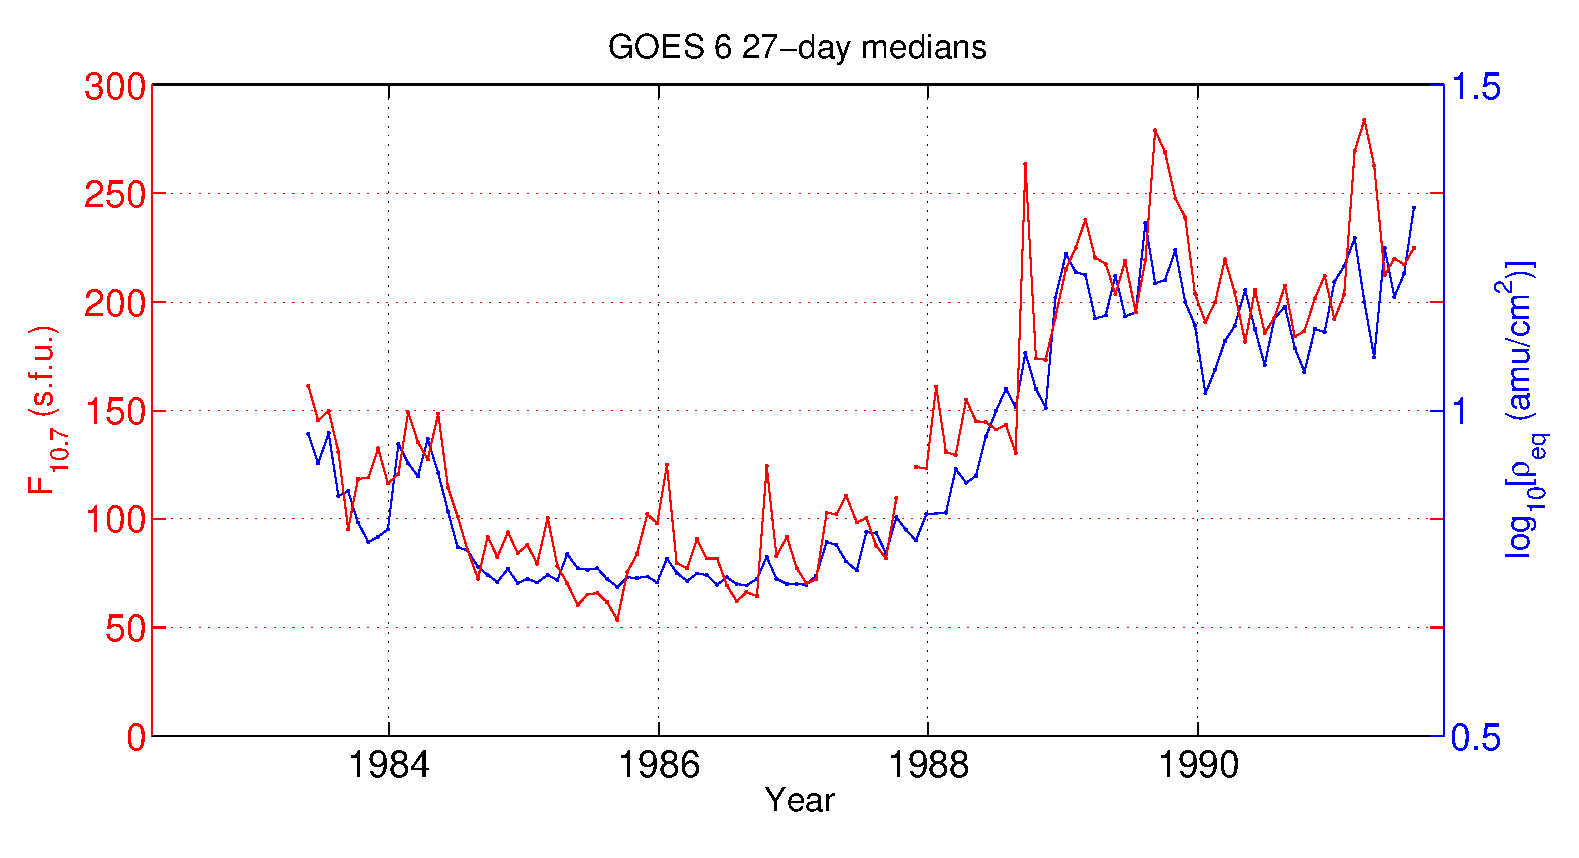
\includegraphics[width=0.85\linewidth]{Figures/F107MD27d-GOES6}
		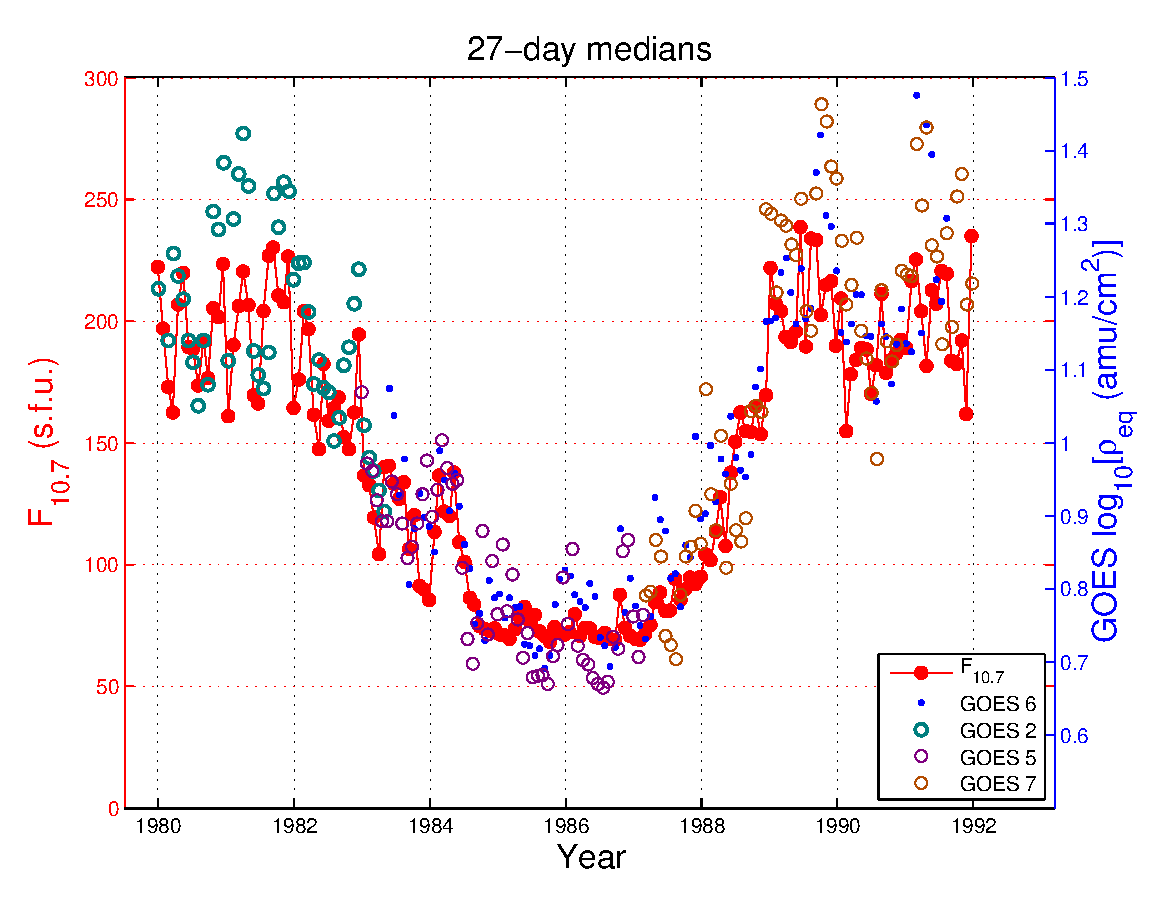
\includegraphics[width=0.85\linewidth]{Figures/F107MD27d-all}
	\caption{Top: Comparing $F_{10.7\_27d}$ and $log(\rho_{eq\_27d})$ using GOES 6 data. Bottom: Same as top, but all available satellites}
	\label{fig:F107rhoeq27dcomparison}
\end{figure}

\begin{figure}[htp!]
	\centering
	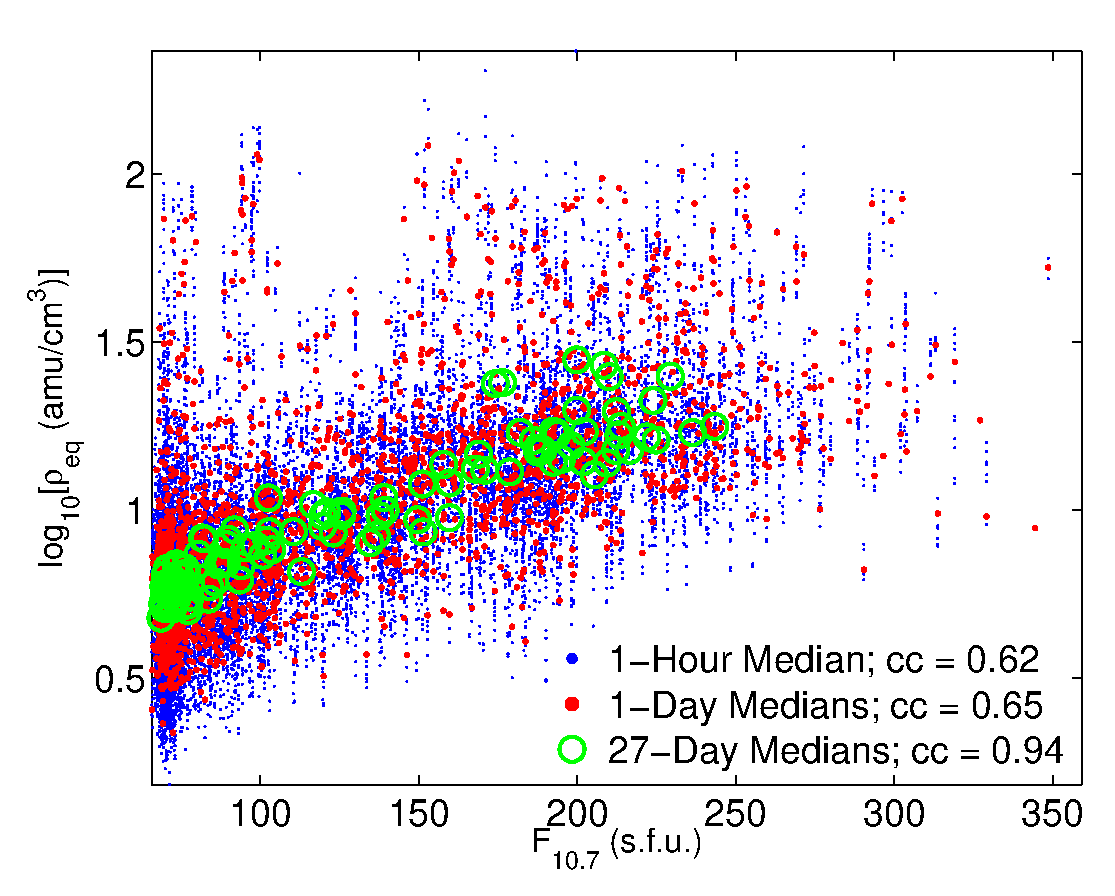
\includegraphics[width=0.55\linewidth]{Figures/ccplot-GOES6}
	\caption{\f\ and $log(\req)$ correlation at varying time scales}
	\label{fig:ccplot}
\end{figure}


The dependence was then analyzed in a more nonlinear manner by investigating the behavior of storms under different $F_{10.7}$ conditions. The hypothesis being that solar activity would drive both geomagnetic storms and, consequently, \req. By separating storms into bins based on the median value of \f, then breaking those two bins into another two bins each separated by their respective medians, a profile of all storm behavior based on \f\ is obtained. Figure \ref{fig:HighLowF107rhoeq} shows the results of this across the events where \dst\ crossed below the $-50$~nT threshold. 

\begin{figure}[htp!]
	\centering
	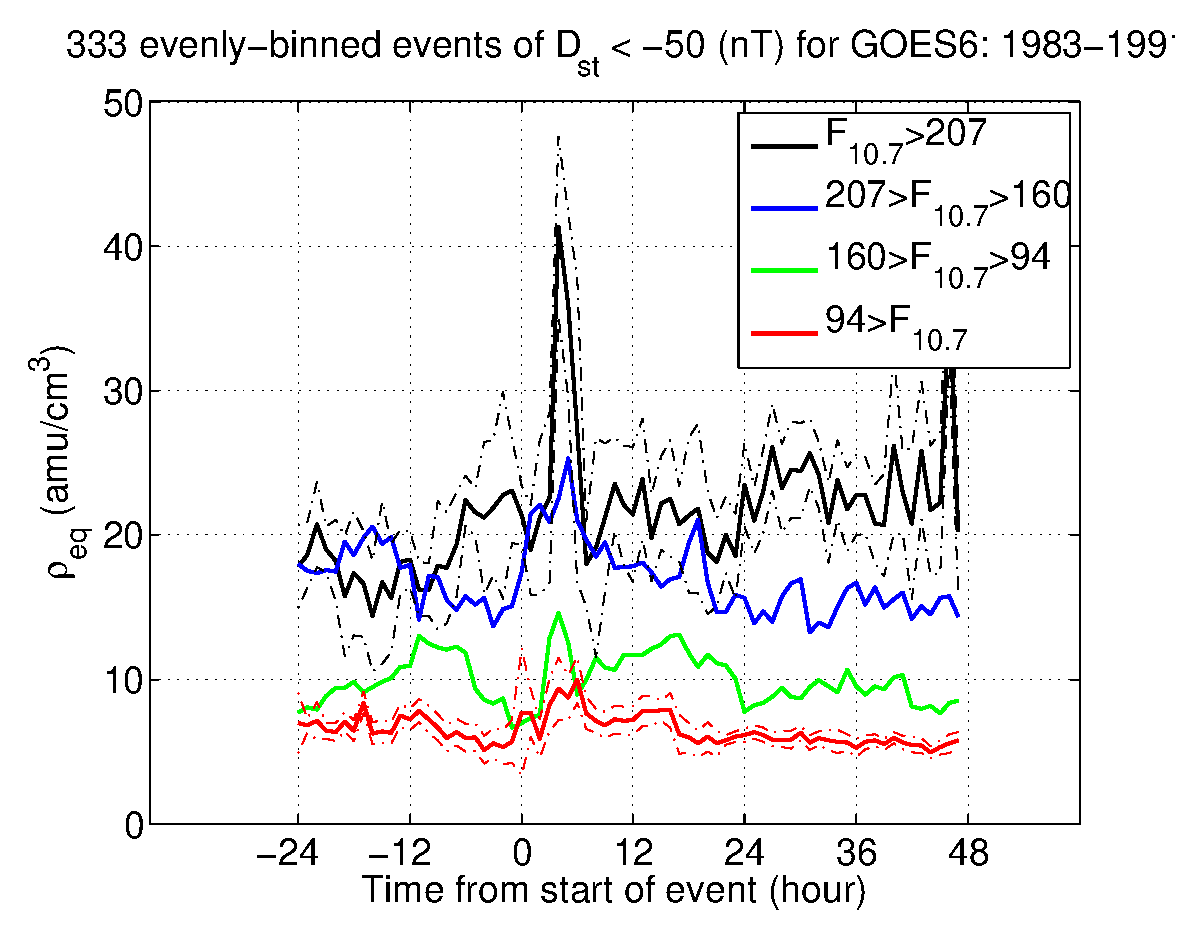
\includegraphics[width=0.7\linewidth]{Figures/HighLowF107rhoeq-Dst50-GOES6-1983-1991}
	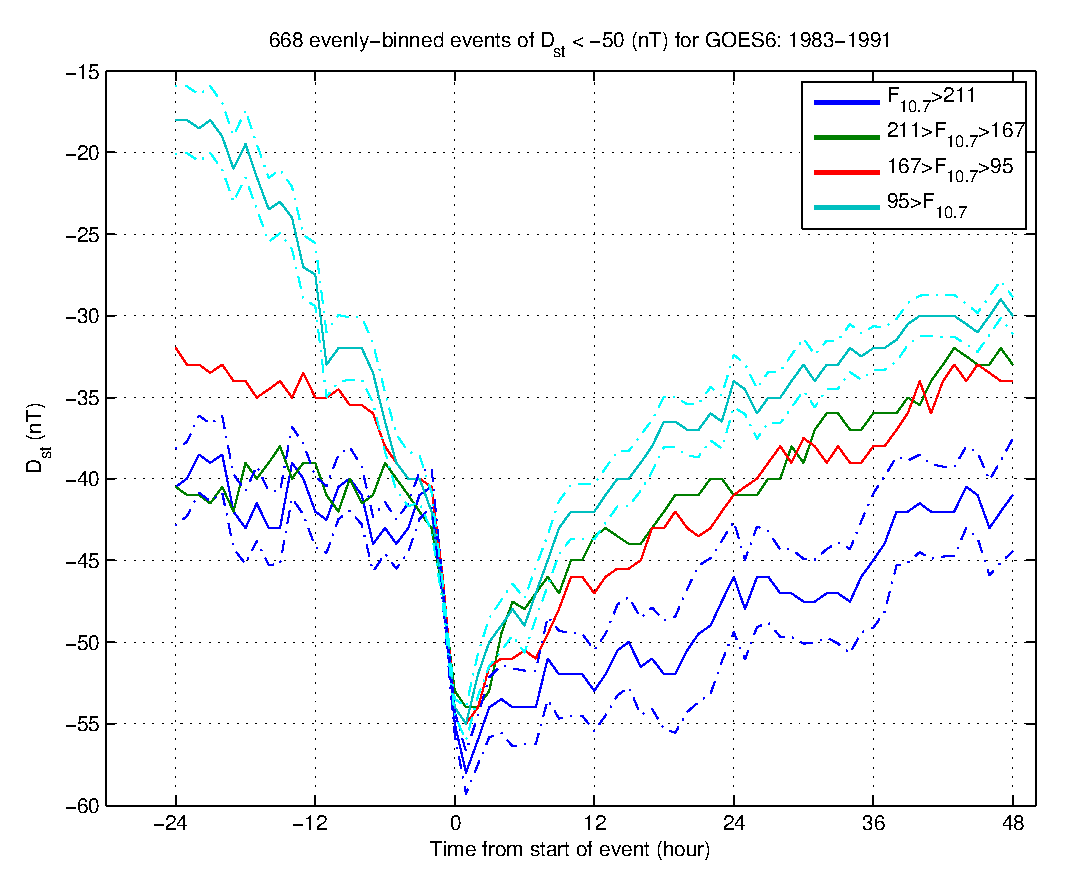
\includegraphics[width=0.7\linewidth]{Figures/HighLowF107Dst-Dst50-GOES6-1983-1991}	
	\caption{\req\ and \dst\ of events binned by median \f\ values. \vinote{Literature search on \f\ and \dst. Temerin and Li \dst\ model. Bz seems to have little impact. }}
	\label{fig:HighLowF107rhoeq}
\end{figure}

Figure \ref{fig:HighLowF107rhoeq}.a shows that \req\ reacts to decreases in \dst, but seemingly only during periods of higher solar activity. Since higher \f\ also correlates with a higher baseline \req, this effect could be due to saturation of the plasmasphere from the increased solar activity. It should also be noted that this trend isn't seen as strongly for all satellites. GOES 2 and 6 show a significant spike and baseline shift, while GOES 7 and 5 lack the significant spike and shift respectively. 

Figure \ref{fig:HighLowF107rhoeq}.b shows that though all events are selected based on a \dst\ threshold, the behavior before and after the storm is affected by \f. For low solar activity events, the \dst\ changes are more sudden and severe, coming from and going back to a more positive baseline. High solar activity events have a longer recovery period.



\section{$B_z$ Dependence}

Similar to the \f\ dependence, tests were done to see if event behavior varied with the $z$-component of the interplanetary magnetic field (IMF). It's well established that the orientation of $B_z$ has a strong correlation with the strength of geomagnetic storms \citep{Takahashi2010SolarCycleVariation}, so events were found based on a threshold of $\req \geq 20~amu/cm^3$. These events were then binned by both the median $B_z$ at and four hours after threshold crossing, and $B_z$ at and four hours before threshold crossing. Figure \ref{fig:RhoBinnedBz} shows both cases.

\begin{figure}[htp!]
	\centering
	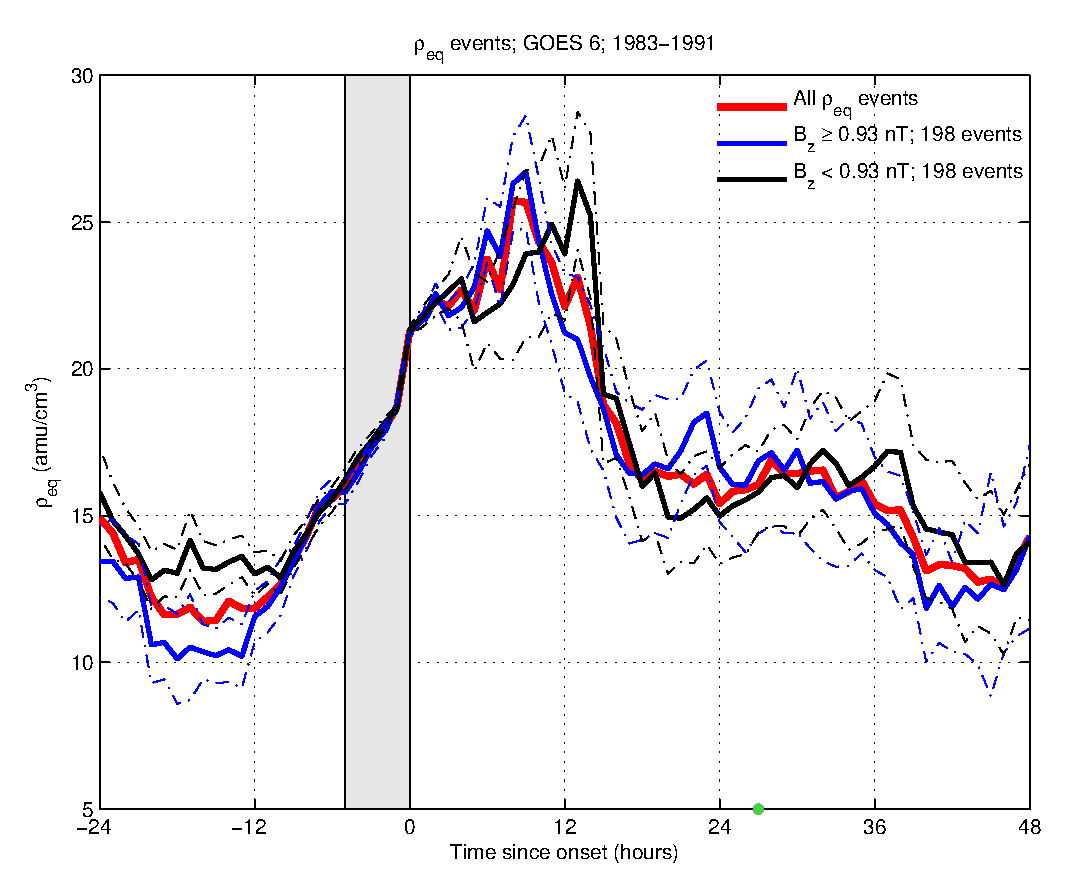
\includegraphics[width=0.7\linewidth]{Figures/RhoBinnedBz-case24-t020-tf25-GOES6}
	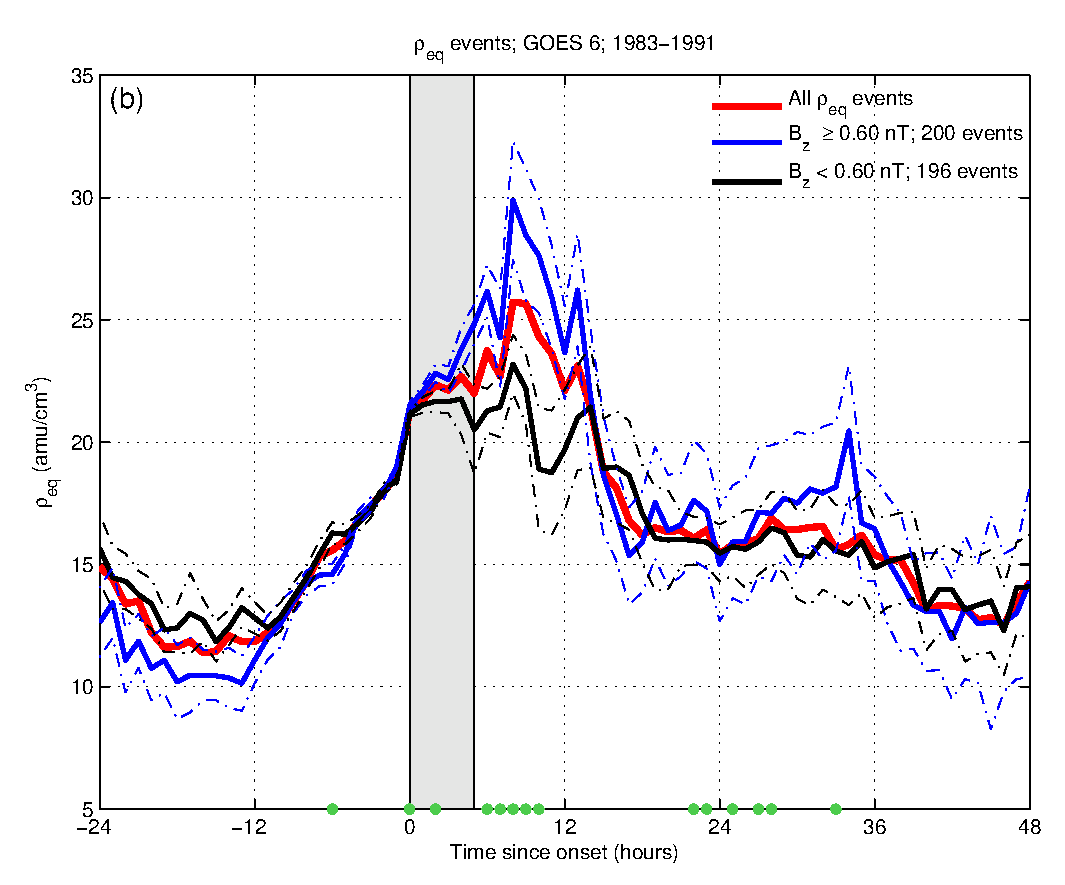
\includegraphics[width=0.7\linewidth]{Figures/RhoBinnedBz-case24-t025-tf30-GOES6}	
	\caption{\req\ events binned by median $B_z$ before and after event onset}
	\label{fig:RhoBinnedBz}
\end{figure}

For each binning method, a two sample t-test was performed for each hour to determine if the samples in each bin had significantly different means from those of the other bin. As there are 73 hours to perform a t-test on, a 95\% confidence interval could be expected to have at least four randomly significant results. Because of this, the one significant t-test result for events binned by pre-onset $B_z$ can not confirm that such a division shows significantly different behaviors, whereas the 14 significant test results for post-onset $B_z$ can be said to show a significant division in behavior between the bins. This physically suggests that the further into a \req\ increase you get, the more $B_z$ orientation impacts the long-term recovery to normal conditions (and indeed moving the window further in time did continue to show significance, but weakly and with no obvious trend). If instead of splitting into equal-number bins, the division is based on positive or negative $B_z$, either time window produces seven or more significant results, but with the added complication that one bin has twice as many samples as the other and may be biased by averaging or the lack thereof. 

\cite{Temerin2002NewModelPredictionDst} discuss the impact of $B_z$ on their model of \dst\ showing a seasonal variation of \dst. Figure \ref{fig:DoYDst} shows how \dst\ seems to vary with day of year (DoY) in our nonlinear models. It seems to support the idea of a seasonal variation, and weakly the idea that $B_z$ also plays a part in that relationship.

\begin{figure}[htp!]
	\centering
	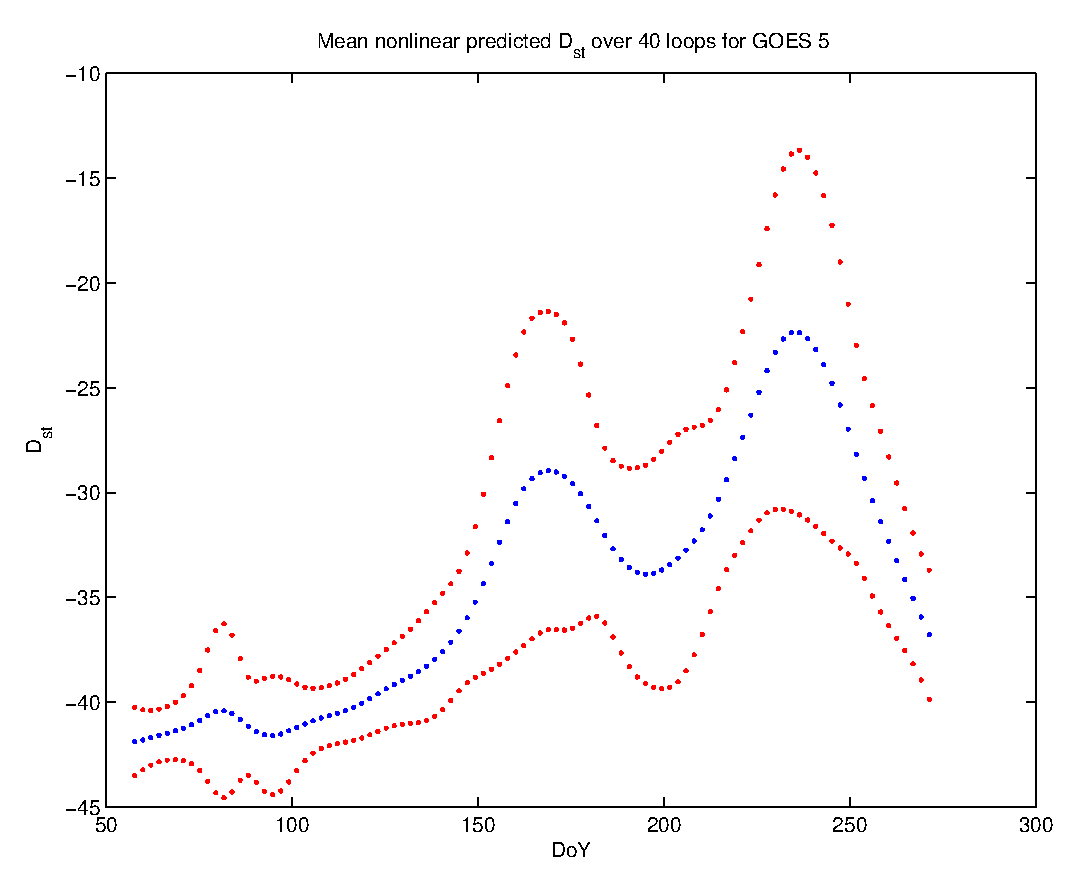
\includegraphics[width=0.7\linewidth]{Figures/NNDoY-Dst-GOES5}	
	\includegraphics[width=0.7\linewidth]{Figures/NNDoY-Bz-Dst-GOES5}
	\caption{\dst\ predicted by nonlinear model of day of year. Bottom: Same, but including a dimension for $B_z$. \vinote{Make non-model version? See/improve DoYDst}}
	\label{fig:DoYDst}
\end{figure}
